\documentclass[]{deedy-resume-openfont}

\begin{document}

%%%%%%%%%%%%%%%%%%%%%%%%%%%%%%%%%%%%%%
%
%     COLUMN ONE
%
%%%%%%%%%%%%%%%%%%%%%%%%%%%%%%%%%%%%%%

\begin{minipage}[t]{0.3\textwidth} 

% ========== 新增的左侧姓名与联系方式 ==========
{\sffamily \fontspec[Path = fonts/lato/]{Lato-Lig}\fontsize{26pt}{30pt}\selectfont 袁中政} \\
\vspace{6pt}
{\color{headings}\fontspec[Path = fonts/raleway/]{Raleway-Medium}\fontsize{10pt}{14pt}\selectfont
\href{mailto:genhz@foxmail.com}{genhz@foxmail.com} \\
+86-131-7311-7610\\
GitHub://  \href{https://github.com/genhz}{\custombold{@genhz}}
}
\vspace{12pt}
% ==============================================

%%%% 利用tikz来定位照片，部分招聘单位可能需要“以貌取人”
\begin{tikzpicture}[remember picture, overlay] 
  % 注意：因为顶部加了姓名，如果照片和文字重叠，可以调整这里的 -4cm（比如改成 -5cm 向下移）
  \node[anchor = north west] at ($(current page.north west)+(+1.8cm,-3cm)$) {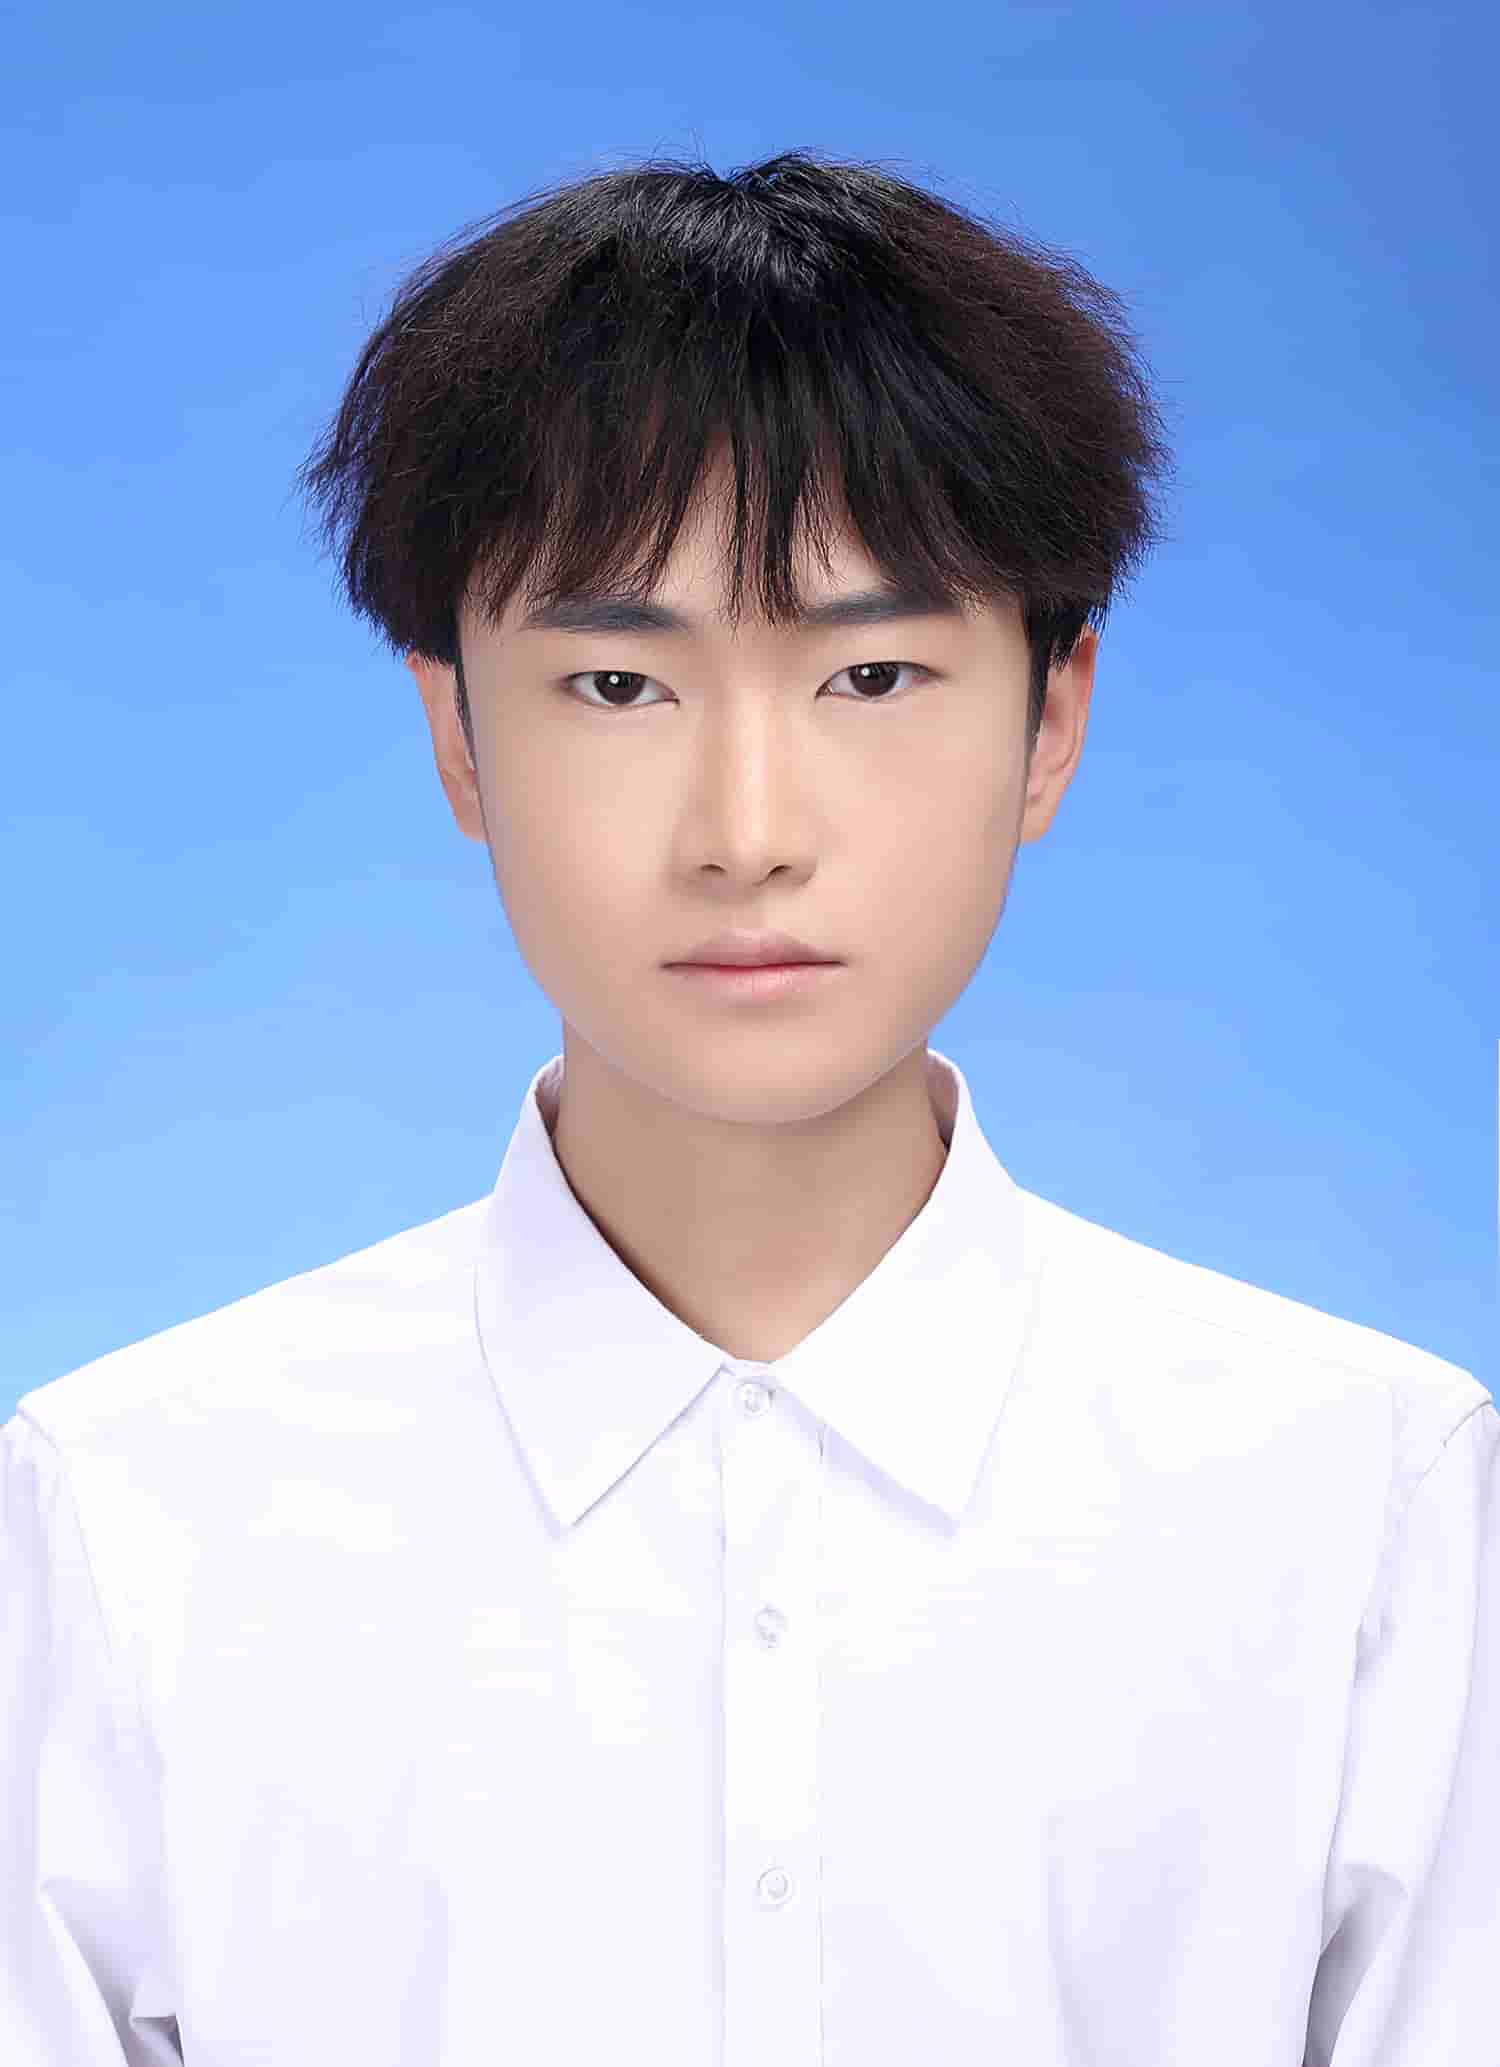
\includegraphics[height=4.2cm]{avatar}};
\end{tikzpicture}%

% 由于顶部增加了姓名信息占据了空间，这里的暴力换行符(~\\)我帮你减少了几个
% 如果你发现“教育背景”依然和照片重叠，可以酌情增加或减少这里的 ~\\
~\\
~\\
~\\
~\\
~\\
~\\
~\\

\section{教育背景} 
\subsection{山东大学}
\descript{计算机技术|硕士研究生}
\location{2024.9-至今}
\subsection{哈尔滨理工大学}
\descript{软件工程|本科}
\location{2020.9-2024.7}
\sectionsep


\section{自我介绍}
\subsection{应聘 \quad 算法实习生}
\quad \\
24岁，来自山东潍坊，硕士在读，研究方向图联邦学习，具备扎实的深度学习与后端开发基础。
有完整AI系统开发经验（模型训练 + 后端部署 + 前端展示）。
发表SCI论文并参与多个科研项目，具备良好的工程实现与科研能力。
\sectionsep

\section{研究方向}
\textbullet{} 图联邦学习 \\
\textbullet{} 医学图像分割

%%%%%%%%%%%%%%%%%%%%%%%%%%%%%%%%%%%%%%
%     LINKS
%%%%%%%%%%%%%%%%%%%%%%%%%%%%%%%%%%%%%%

% \section{链接} 
% GitHub://  \href{https://github.com/fuujiro}{\custombold{@fuujiro}} \\
% Blog://  \href{https://blog.fuujiro.com}{\custombold{fuujiro's island}} \\
% 知乎:// \href{https://www.zhihu.com/people/fuujiro/activities}{\custombold{fuujiro}} \\
% \sectionsep

%%%%%%%%%%%%%%%%%%%%%%%%%%%%%%%%%%%%%%
%     COURSEWORK
%%%%%%%%%%%%%%%%%%%%%%%%%%%%%%%%%%%%%%
\section{荣誉奖项}
\textbullet{} 黑龙江省三好学生\\
\textbullet{} 黑龙江省优秀毕业生\\
\textbullet{} 哈尔滨理工大学三好学生\\
\textbullet{} 哈尔滨理工大学优秀毕业生\\
\textbullet{} 国家励志奖学金\\
\textbullet{} 东北三省数学建模联赛·二等奖 \\
\textbullet{} 蓝桥杯A组·省级三等奖 \\
\textbullet{} "互联网＋"大赛·省级银奖 \\
\textbullet{} "互联网＋"大赛·省级铜奖 \\
\textbullet{} 校级一等奖学金和三好学生若干\\
% \sectionsep

% \section{资格证书与外语水平}
\textbullet{} 软件设计师 \\
\textbullet{} CET 4 \\
\sectionsep



%%%%%%%%%%%%%%%%%%%%%%%%%%%%%%%%%%%%%%
%     SKILLS
%%%%%%%%%%%%%%%%%%%%%%%%%%%%%%%%%%%%%%

\section{专业技能}
\textbullet{} Python \textbullet{} Java \textbullet{}  C/C++\\
\textbullet{} PyTorch \textbullet{} PyTorch Geometric (PyG) \\
\textbullet{} SpringBoot \textbullet{} Vue \textbullet{} MySQL \\
\sectionsep

%%%%%%%%%%%%%%%%%%%%%%%%%%%%%%%%%%%%%%
%
%     COLUMN TWO
%
%%%%%%%%%%%%%%%%%%%%%%%%%%%%%%%%%%%%%%

\end{minipage} 
\hfill
\begin{minipage}[t]{0.66\textwidth} 

%%%%%%%%%%%%%%%%%%%%%%%%%%%%%%%%%%%%%%
%     EXPERIENCE
%%%%%%%%%%%%%%%%%%%%%%%%%%%%%%%%%%%%%%
\section{实习经历}

\runsubsection{北京有研亿金新材料有限公司}
\descript{ 生产运营部 }
\location{2023.10 – 2024.05 | 质量管理系统开发}
\vspace{\topsep} % Hacky fix for awkward extra vertical space
\begin{tightemize}
\item 参与公司质量管理系统的后端开发，负责部分核心业务模块（如质量检测数据管理/流程管理）的设计与实现。
\item 基于 .NET Web API 构建后端服务，完成数据建模与接口开发。
\end{tightemize}
\sectionsep


% \section{在校经历}

% \runsubsection{校外项目}
% \descript{| 姜家庄家谱管理系统 }
% \location{2025.06 – 2026.03 | 核心开发人员}
% \vspace{\topsep} % Hacky fix for awkward extra vertical space
% \begin{tightemize}
% \item 负责家谱管理系统核心模块开发，包括家族关系管理、村志信息管理及用户权限管理。
% \item 基于 Vue + SpringBoot + MyBatis Plus 实现前后端分离架构，设计 RESTful API 并完成数据库建模。
% \end{tightemize}
% \sectionsep

\section{科研经历}

\runsubsection{图联邦学习算法研究}
\descript{| 半异步广义类别发现图联邦学习 }
\location{2024.09 – 至今 | 山东大学}
\vspace{\topsep}
\begin{tightemize}
\item \textbf{核心科研成果产出（两篇一区在审）：} 基于异步通信优化与广义类别发现双重维度的理论突破及工程验证，共主导撰写并投递了两篇高质量学术论文，目前均在中科院/JCR一区顶级期刊审稿阶段。
\item \textbf{核心科研成果产出（两篇一区在审）：} 基于异步通信优化与广义类别发现双重维度的理论突破及工程验证，共主导撰写并投递了两篇高质量学术论文，目前均在中科院/JCR一区顶级期刊审稿阶段。
\end{tightemize}
\sectionsep

\runsubsection{国家级大学生创新创业项目}
\descript{| “ThirdEye AI”眼底视网膜图像自动分级分割系统 }
\location{2022.07 – 2023.05 | 第一负责人 · 优秀结题}
\vspace{\topsep} % Hacky fix for awkward extra vertical space
\begin{tightemize}
% \item 负责眼底视网膜图像分割与分级算法的设计与实验，基于深度学习模型（如 U-Net 等）进行优化与改进。
% \item 搭建完整实验流程，包括数据预处理、模型训练、评估指标设计（如 Dice / IoU）等。
\item 以第一作者发表 SCI 二区论文 1 篇，并参与发表多篇相关研究论文。
\item 基于 Django 独立开发系统平台，实现模型在线推理与结果可视化，并完成部署与答辩展示。
\end{tightemize}
\sectionsep

\runsubsection{国家级大学生创新创业项目}
\descript{| 基于余弦退火和快照集成的U-Net网络的肝脏CT自动分割优化 }
\location{2022.07 – 2022.05 | 成员 · 优秀结题}
\vspace{\topsep} % Hacky fix for awkward extra vertical space
\begin{tightemize}
\item 基于 U-Net 模型进行肝脏 CT 图像分割实验，参与 baseline 搭建与训练流程设计。
% \item 引入余弦退火学习率调度与快照集成（Snapshot Ensemble）策略，提高模型泛化能力。
\end{tightemize}
\sectionsep

\sectionsep


\section{学术论文}
[1] Yuan Z, Guo L, Li X, et al. FedSA-GCL: A Semi-Asynchronous Federated Graph Learning Framework with Personalized Aggregation and Cluster-Aware Broadcasting[J]. arXiv preprint.(中科院一区top在审)

[2] Guo L, Yuan Z, Li X, et al. DFed-SST: Building Semantic-and Structure-aware Topologies for Decentralized Federated Graph Learning[J]. arXiv preprint.(JCR一区在审)

[3] Yuan Z, Wang J, Xu Y, et al. CC-TransXNet: a hybrid CNN-transformer network for automatic segmentation of optic cup and optic disk from fundus images[J]. Medical & Biological Engineering & Computing, 2025, 63(4): 1027-1044. 

[4] Wang J, Zhou L, Yuan Z, et al. Mic-net: multi-scale integrated context network for automatic retinal vessel segmentation in fundus image[J]. Mathematical Biosciences and Engineering, 2023, 20(4): 6912-6931.

[5] Wang X, Guo L, Yuan Z, et al. Towards eye-tracking-based technology on sight interpretation performance improvement[J]. Journal of Mechanics in Medicine and Biology, 2022, 22(09): 2240058.

[6] Sun Y, Li X, Liu Y, et al. A lightweight dual-path cascaded network for vessel segmentation in fundus image[J]. Mathematical Biosciences and Engineering, 2023, 20(6): 10790-10814.


\end{minipage} 
\end{document}